\chapter{实验结果与分析}

前面章节详细介绍了本文的进化算法硬核布局的原理与实现方式,并介绍了RapidLayout FPGA实现框架的
原理与工作流程。本章通过对比实验设计研究进化算法布局与模拟退火、解析布局等
方法性能的比较,并验证迁移学习的有效性。
首先,本章介绍实验中涉及的FPGA器件与对比算法,然后介绍实验的编程实现、运行环境、参数确定等实验细节。
本章设计了多种可视化方法,展示本文提出的进化布局算法与state-of-the-art方法
的性能、收敛过程对比,并详细讨论了流水线级数对时钟频率的影响。
最后,本章评估RapidLayout的迁移学习性能并展示布局结果。

\section{Xilinx UltraScale+ FPGA 介绍}

% 列出资源表
\begin{table}[h]
	\centering
	\caption{实验器件 Xilinx UltraScale+ Virtex 资源列表}		
	\label{tab:fpg}
	\begin{tabular}{c|c c c c c c}
		\toprule[2pt]
        型号 	& SLR数目 & DSP 数目 & BRAM 数目 & URAM 数目 & Flip-Flops(K) & LUTs(K)	\\
        \midrule[2pt]
        VU3P   & 1       & 2280    & 1440     & 320       & 788               & 394 \\
        \hline 
        VU5P   & 2       & 4560    & 2880     & 640       & 1201              & 601 \\
        \hline
        VU7P   & 2       & 4560    & 2880     & 640       & 1576              & 788 \\
        \hline
        VU9P   & 3       & 6840    & 4320     & 960       & 2364              & 1182 \\
        \hline
        VU11P  & 3       & 9216    & 4032     & 960       & 2592              & 1296 \\
        \hline 
        VU13P  & 4       & 12288   & 5376     & 1280      & 3456              & 1728 \\
        \bottomrule[2pt]
	\end{tabular}
\end{table}

表\ref{tab:fpg}列出了本文实验中使用的FPGA及其计算资源。UltraScale+ 是Xilinx推出的高端14/16nm系列FPGA,搭载了
DSP48,Block RAM 和 Ultra RAM 三种计算存储硬核资源。RapidLayout FPGA布局框架是面向UltraScale+系列FPGA而设计的,
支持除了HBM(High-Bandwidth Memory)型号以外的全部FPGA。

\section{对比布局算法}
% 几个对比算法,近似处理的做法
本文选取了多个布局算法作为对比实验,包括:(1)模拟退火算法; (2)基于模拟退火的标准FPGA实现工具Versatile Place and Route~\cite{vtr2014};
(3) State-of-the-art 解析布局算法 UTPlaceF~\cite{li2017utplacef}; (4)单目标遗传算法; (5)RapidWright内部布局引擎(基于退火~\cite{lavin2018rapidwright};
(6)Vivado解析布局引擎。本节阐述以上对比实验的原理简介与实现方法。

\subsection{模拟退火算法 Simulated Annealing}
\label{sec:sa}

模拟退火算法(Simulated Annealing)是一种基于概率的启发式搜索优化算法,它将系统模拟为高温熔化材料逐渐凝固的过程,每一轮迭代对当前系统状态
做出随机变化,通过温度函数控制接受该随机改变的概率,经常被用在离散系统的优化,FPGA布局问题是其经典应用之一。退火算法已经被证明,
对于FPGA布局问题在无限长的时间内可以保证收敛到全局最优值。但是,退火算法的收敛速度和结果质量极大受到冷却进度表(Cooling Schedule)的影响:
冷却速度过快会导致系统收敛到局部最优点,速度过慢则会导致收敛时间显著变长。一般来说,冷却进度表的确定是与优化问题相关的,也就是
需要针对具体优化问题调节参数。本文中使用Opt4J优化框架的退火优化引擎,用Java实现了FPGA硬核布局的模拟退火搜索方法。
第\ref{sec:cooling}节对于冷却进度表的确定进行实验并给出了最优结果。由于退火算法仅支持单目标优化,本文将提出的两个目标函数乘积作为
退火算法的优化目标函数。

\subsection{Versatile Place and Route}

Versatile Place and Route (VPR) 是多伦多大学提出的Verilog-to-Route(VTR)~\cite{vtr2014} FPGA实现框架的布局布线工具,是学术界最常用的
标准对比基线。VPR基于模拟退火算法,提出了一种线性阻塞(linear congestion)目标函数改进,其形式如式(\ref{eq:vpr})确定。

\begin{equation}
Cost = \sum_{n=1}^{N_{nets}} q(n) [ \frac{bb_x(n)}{C_{av,x}(n)} + \frac{bb_y(n)}{C_{av,y}(n)} ] 
\label{eq:vpr}
\end{equation}

其中求和是对于所有的信号线,$bb_x$ 和 $bb_y$ 代表每个信号线边界框的宽和高,$q(n)$ 是对实际线长估计的补偿值,$C_{av,x}$ 和 $C_{av,y}$
是横纵方向平均的布线通道容量。本文采用了最新的VPR 7.0 Official Release 二进制文件作为对比。由于VPR使用的架构与网表格式与RapidWright
不同,本文基于Python开发了以下工具:(1)将Xilinx UltraScale+ VU11P 架构转化为 \texttt{architecture.xml} 架构信息转化工具;
(2)将本文使用的脉动阵列网表转化为 Berkeley Logic Interchange Format 的工具,生成 \texttt{conv\_model.blif} 文件;
(3)将VPR布局结果转化为RapidWright和Vivado支持的XDC格式的转换工具。
以上工具链均与RapidLayout集成,在对比实验时由RapidLayout自动调用。

\subsection{UTPlaceF 解析算法布局工具}

UTPlaceF是目前最先进的解析布局算法工具,由德克萨斯大学奥斯汀分校~\cite{li2017utplacef}提出,并于ISPD2016 Routing-Aware Placement Contest获得一等奖。
UTPlaceF使用HPWL(Half-Parameter Wirelength)作为目标函数,其形式为:
\begin{equation}
 HPWL(x,y) = \sum_{e \in E} {max_{i,j \in e} |x_i-x_j| + max_{i,j \in e} |y_i-y_j|} 
\end{equation}

其中$E$为全部信号线,$x, y$为信号线连接的全部计算单元(cell)。UTPlaceF使用欧氏距离平方对HPWL近似从而使其可导,
然后使用Quadratic Programming求解布局结果。本文使用UTPlaceF TCAD Version 公开的二进制文件进行对比实验。由于
UTPlaceF 使用 Extended BookShelf Format 作为架构和逻辑网表的定义格式,本文同样开发了网表和布局结果的转换工具,
与RapidLayout集成,自动调用。

{\bf 架构近似:} 由于UTPlaceF仅面向UltraScale架构~\cite{li2017utplacef},其架构定义不包括Ultra RAM硬核。因此,本文根据硬核大小做出如下近似:
UltraScale+ RAMB18 $\rightarrow$ UltraScale DSP48, 
UltraScale+ URAM288 $\rightarrow$ UltraScale RAMB36,
并保持硬核数量、列分布与UltraScale+ VU11P FPGA相同。

\subsection{遗传算法 Genetic Algorithm}

遗传算法(Genetic Algorithm, GA)是最基本的进化算法。本文采用Opt4J~\cite{opt4jpaper} Java 优化框架实现了单目标的GA硬核布局引擎。遗传算法采用
最基本的交叉(Cross-over)和变异(Mutation)产生新的可行解,但仅支持单一目标函数。本文采用与NSGA-II相同的问题建模,目标函数为
卷积计算单元最大边界框尺寸,基因型设计与参数设置和NSGA-II保持相同。本实验的目的在于说明多目标优化对布局结果质量提升的影响。

\subsection{RapidWright布局引擎}

RapidWright支持基于Modular Design~\cite{lavin2018rapidwright}的实现方式,可以将一个卷积运算单元包装为一个Module,使用内置的退火引擎进行布局。
但实际试验结果如图\ref{fig:rapidwright_baseline}所示,无法在VU11P FPGA上完成对480个卷积运算单元的布局。失败的原因在于:
RapidWright首先对Module分析,得到整个FPGA上所有的可布局位置。但由于硬核的列分布不规律,RapidWright仅能发现同列
的可布局位置。在图\ref{fig:rapidwright_baseline}中,RapidWright仅发现了12个可布局位置,因此其退火引擎无法
给出对于480个卷积计算单元的合法布局结果。

\begin{figure}[h]
	\centering
	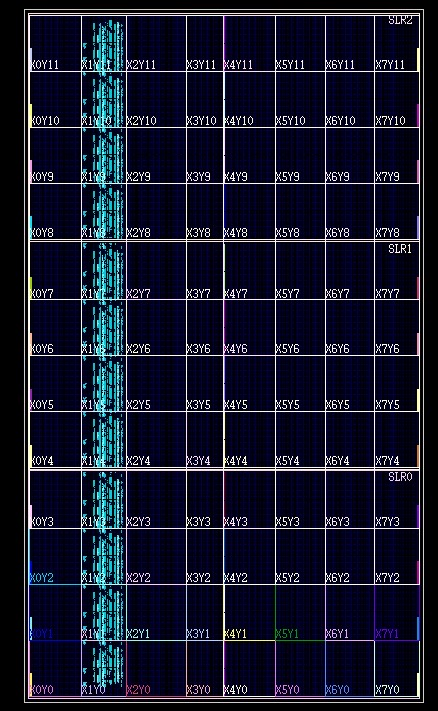
\includegraphics[width=0.5\textwidth]{figure/rapidwright_baseline.png}
	\caption{RapidWright退火布局引擎在VU11P FPGA上的布局结果} 
	\label{fig:rapidwright_baseline}
\end{figure}


\subsection{Vivado 解析布局引擎}

Vivado的布局引擎是多目标的解析布局引擎。但对于本文中的480个卷积计算单元无法在不通过手工布局的情况下给出可布线的布局结果。

\begin{itemize}
    \item 图\ref{fig:overview} (a) 展示了Vivado在不给出手工布局的情况下仅依赖内置的解析布局引擎得到的尝试布线结果,图中的
    红色连线表示布线失败的信号。由于Vivado给出的布局结果质量差,布线阶段纵向布线资源耗尽所以FPGA实现失败。
    
    \item 图\ref{fig:overview} (b) 展示了Vivado在给出全部硬核布局的实现结果。由于Vivado无法自行通过解析布局引擎完成
    设计布局,所以需要通过手工设计的方式将480个卷积运算单元的所有硬核布局位置确定,并通过XDC Constraint的方式输入Vivado,
    Vivado仅完成控制逻辑的布局。手工设计的方式通常需要消耗几周的时间试错才能最终得到可以达到650 MHz时钟频率的结果,所需的
    人力工作量巨大。尽管如此,在给出硬核布局的情况下Vivado的完整实现仍需5--6小时才可完成。与此相对的是,RapidLayout可
    以自动发现硬核布局,保证达到650 MHz以上的时钟频率,不但避免了大量的人力工作,而且整体实现时间缩短到1小时左右。

\end{itemize}

Vivado的布局实验再次说明了高硬核利用率的设计和不规则的硬核大小与分布,为布局布线带来了很大的难度。即使是Vivado这样成熟的
商业化解析布局引擎也无法自动完成布局。因此,开发RapidLayout基于进化算法的多目标快速布局引擎是有必要的。




\section{实验的编程实现}


\subsection{运行环境}
\begin{table}[h]
	\centering
	\caption{实验测试环境}		
	\label{tab1}
	\begin{tabular}{c|c}
		\toprule[2pt]
        CPU & Intel Xeon Gold 6230 40-Thread\\
        \hline
		操作系统 & Ubuntu 16.04 LTS \\
		\hline                                        
		内存 	& 128 GB	\\
		\bottomrule[2pt]
	\end{tabular}
\end{table}

\subsection{软件工具}

\begin{table}[h]
	\centering
	\caption{实验软件工具}		
	\label{tab2}
	\begin{tabular}{c|c}
		\toprule[2pt]
		RapidWright 	& 2019.12 Beta Pre-release	\\
        \hline                                         
        Vivado Design Suite	&  2018.3 \\
        \hline
        Opt4J~\cite{opt4jpaper}  &  3.1.4 2015-release \\
        \hline
        Apache Commons Math Optimization Library~\cite{apache} & 3.4 \\
        \bottomrule[2pt]
	\end{tabular}
\end{table}

表\ref{tab2}列出了本文实验使用的软件工具。RapidLayout基于RapidWright用Java和Python开发,其中NSGA-II, 模拟退火,
单目标遗传算法布局引擎使用Java的Opt4J优化库实现。对大规模优化问题改进的CMA-ES布局算法通过Apache Commons 
Math Optimization Library Java数学库实现。辅助性套件中,第\ref{sec:visual}节中展示的可视化工具由Python Matplotlib实现,
针对UTPlaceF, VPR对比实验的网表、架构转换工具由Python实现,布局结果转换工具由Java实现。以上各个套件集成在RapidLayout工具链
之中,通过配置文件控制RapidLayout的工作流和输出,组成了完整的端到端FPGA实现框架。


\section{实现细节与敏感度分析}

本节详细阐述模拟退火,CMA-ES,NSGA-II算法的参数选取与敏感度分析,通过实验验证其合理性并得出结论。

\subsection{模拟退火参数确定}
\label{sec:cooling}

通过第\ref{sec:sa}节对模拟退火算法的分析可知,冷却进度表很大程度影响退火的收敛速度与结果质量。因此,本节通过
实验来验证不同冷却进度表对收敛速度与结果的影响程度,并选取最优参数进行与进化算法的对比实验。

\begin{figure}[h]
	\centering
	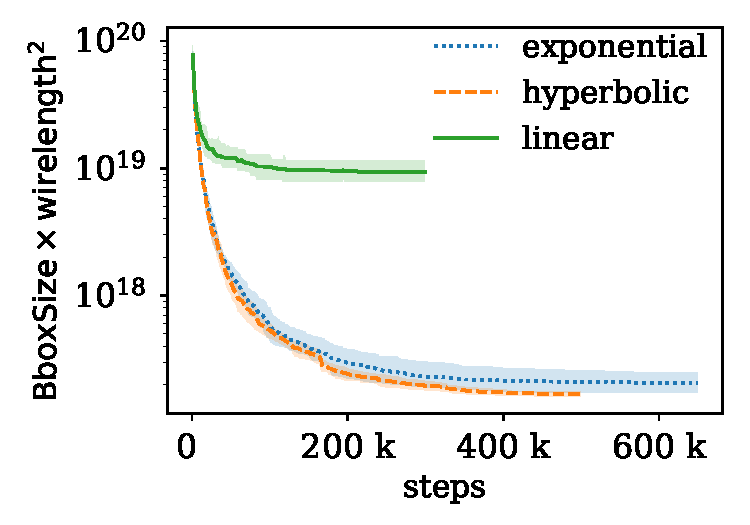
\includegraphics[width=0.8\textwidth]{figure/Annealing-Tuning}
	\caption{模拟退火布局算法在指数、双曲、线性三种类型冷却进度表条件下的目标函数收敛进程} 
	\label{fig:annealing-tune}
\end{figure}

图\ref{fig:annealing-tune}展示了模拟退火算法分别在指数、双曲、线性三种类型的冷却进度表下目标函数的
收敛过程。实验过程中,三种冷却进度表分别选用了十组参数组合,并使用相同的early-stopping标准。
从图\ref{fig:annealing-tune}观察可以得知:
\begin{itemize}
    \item 冷却进度表类别的不同对收敛的影响大于其内部参数的变化。
    \item 线性冷却进度表收敛结束最快,但停止在了局部最小值。
    \item 指数冷却进度表能够达到近似全局最优,但所花时间过长。
    \item 双曲线冷却进度表表现最优,所花时间少与指数函数而能够达到近似全局最优,因此选择双曲线冷却进度表
    作为模拟退火布局引擎的冷却进度,并选择取得收敛后目标函数值最小的一组参数作为默认参数。
\end{itemize}


\subsection{CMA-ES敏感度分析}

\begin{figure}[h]
	\centering
	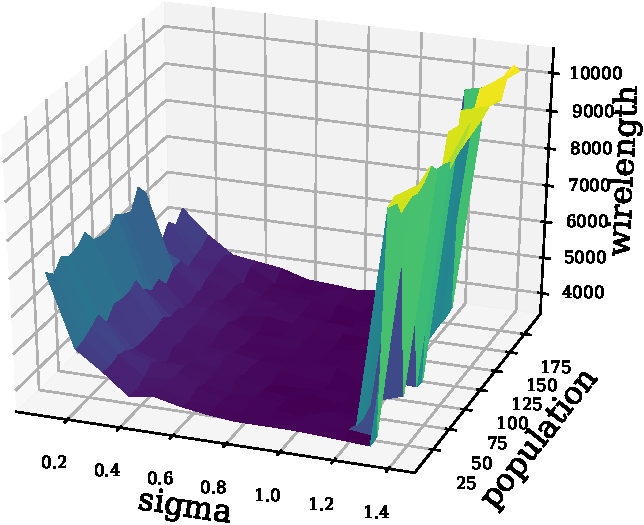
\includegraphics[width=0.6\textwidth]{figure/cma_sensitivity-crop}
	\caption{CMA-ES敏感度分析,改变sigma与population对收敛线长的影响} 
	\label{fig:sensitivity}
\end{figure}

CMA-ES有两个主要的可选参数,一个是$\sigma$初始步长,另一个是采样数population。$\sigma$ 对CMA-ES的优化
过程影响主要有两点:(1)如果$\sigma$设置过小,则容易陷入局部最小值;(2) 如果$\sigma$设置过大,则容易造成
结果不收敛。实验中采取了$\sigma \in [0.1 : 0.1 : 1.5]$ 和 $population \in [20 : 10 : 180]$ 的参数
组合范围,每一组参数运行CMA-ES布局算法10次,取最小值作为该组合的最优表现。得到实验结果如图\ref{fig:sensitivity}
所示,可以观察到$\sigma > 1.2$会导致结果难以收敛,而$\sigma < 0.4$则会收敛至局部最小值,符合对CMA-ES的
分析。而population的改变对优化效果影响不大,因此选择较小的$population=30$作为默认参数,以加快CMA-ES的优化
进程。

\subsection{NSGA-II Reduced}

图\ref{fig:genotype}介绍了本文的“三段”结构基因型设计,分别是Distribution, Location, 和Mapping。
Distribution指定了布局任务选用的硬核在列中的分布,确定了每列选择硬核的个数;Location在此基础上
确定每一个硬核在列中的位置,从而完全确定被选中硬核的物理位置;Mapping在选中位置的基础上规定逻辑硬核与
物理位置的对应关系,从而完全确定一个布局可行解。这种“三段”结构的基因型可以充分表达问题的解空间,为
搜索到全局最优解提供了足够的自由度。

本节提出一种trade-off的思路,取消三个子基因型中的Distribution和Location, 按照均匀分布的方式将
选取硬核的数目分配到各列,再从下至上依次以“堆叠”的方式选取硬核位置。这样,仅优化逻辑硬核与物理位置
的对应关系,意味着放弃了一部分解空间,减小了搜索的自由度,来加速搜索过程。本文将这种仅优化
Mapping部分基因型的NSGA-II算法称为NSGA-II Reduced, 并采用与NSGA-II相同的参数设置进行性能对比实验。


\section{实验设置以及实验结果}

本章以上小节详细介绍了对比实验的原理与最优参数选取方法,本节在此内容的基础上
进行所有算法的布局性能对比实验,性能指标包括:运行时间、目标函数、收敛稳定程度、
布线后设计的时钟频率,以及达到URAM上限650 MHz时钟频率所需的流水线寄存器开销。
最后,本节展示RapidLayout的迁移学习性能,即布局结果迁移到不同型号FPGA的能力。

\subsection{实验设置}
% 各个模型配置,可以列张表

\begin{table}[h]
	\centering
	\caption{实验参数设置}		
	\label{tab:param}
	\begin{tabular}{c|l}
		\toprule[2pt]
		布局算法 	& 参数设置	\\
        \midrule[2pt]                                         
        NSGA-II	&  population=50, mutation=0.99\\
        \hline
        NSGA-II(Red)  & population=50, mutation=0.99  \\
        \hline
        CMA-ES &  $\sigma=0.5$, population=30\\
        \hline
        SA & 双曲冷却进程表: $t = t_0 (\frac{t_n}{t_0})^{i/n}$, $t_0=1000$, $t_n=100$\\
        \hline
        GA & population=50, mutation=0.99 \\
        \hline
        VPR & 使用二进制文件,默认参数\\
        \hline
        UTPlaceF & 使用二进制文件,默认参数\\
        \hline
        Manual & 无参数\\
        \bottomrule[2pt]
	\end{tabular}
\end{table}

表\ref{tab:param}中列出了布局性能对比实验所有方法的参数设置。由于RapidWright无法产生布局结果,所以不纳入性能对比实验;
Manual表示手工布局结果,也就是人工设计480个卷积计算单元硬核在VU11P FPGA的布局结果,以XDC Constraints的形式输入Vivado
进行对比实验。另外需要说明的是,由于UTPlaceF 和 VPR 布局实验无法设置式\ref{eq:cascade}中提出的级联约束条件,因此得到的
布局结果不满足Xilinx UltraScale+ 的架构布局布线要求,所以无法完成时钟频率和流水线开销实验,但仍可以衡量其布局结果的
目标函数值。所有对比实验均在同一实验软件和硬件条件下完成。


\subsection{性能对比}

本节对所有优化算法采用了设置随机种子的初始化,每种优化算法运行50次,随机选取其中的10次结果进行完整实现(布局、布线、Vivado报告时钟频率)
对比时钟频率结果。

\begin{figure}[h]
	\centering
	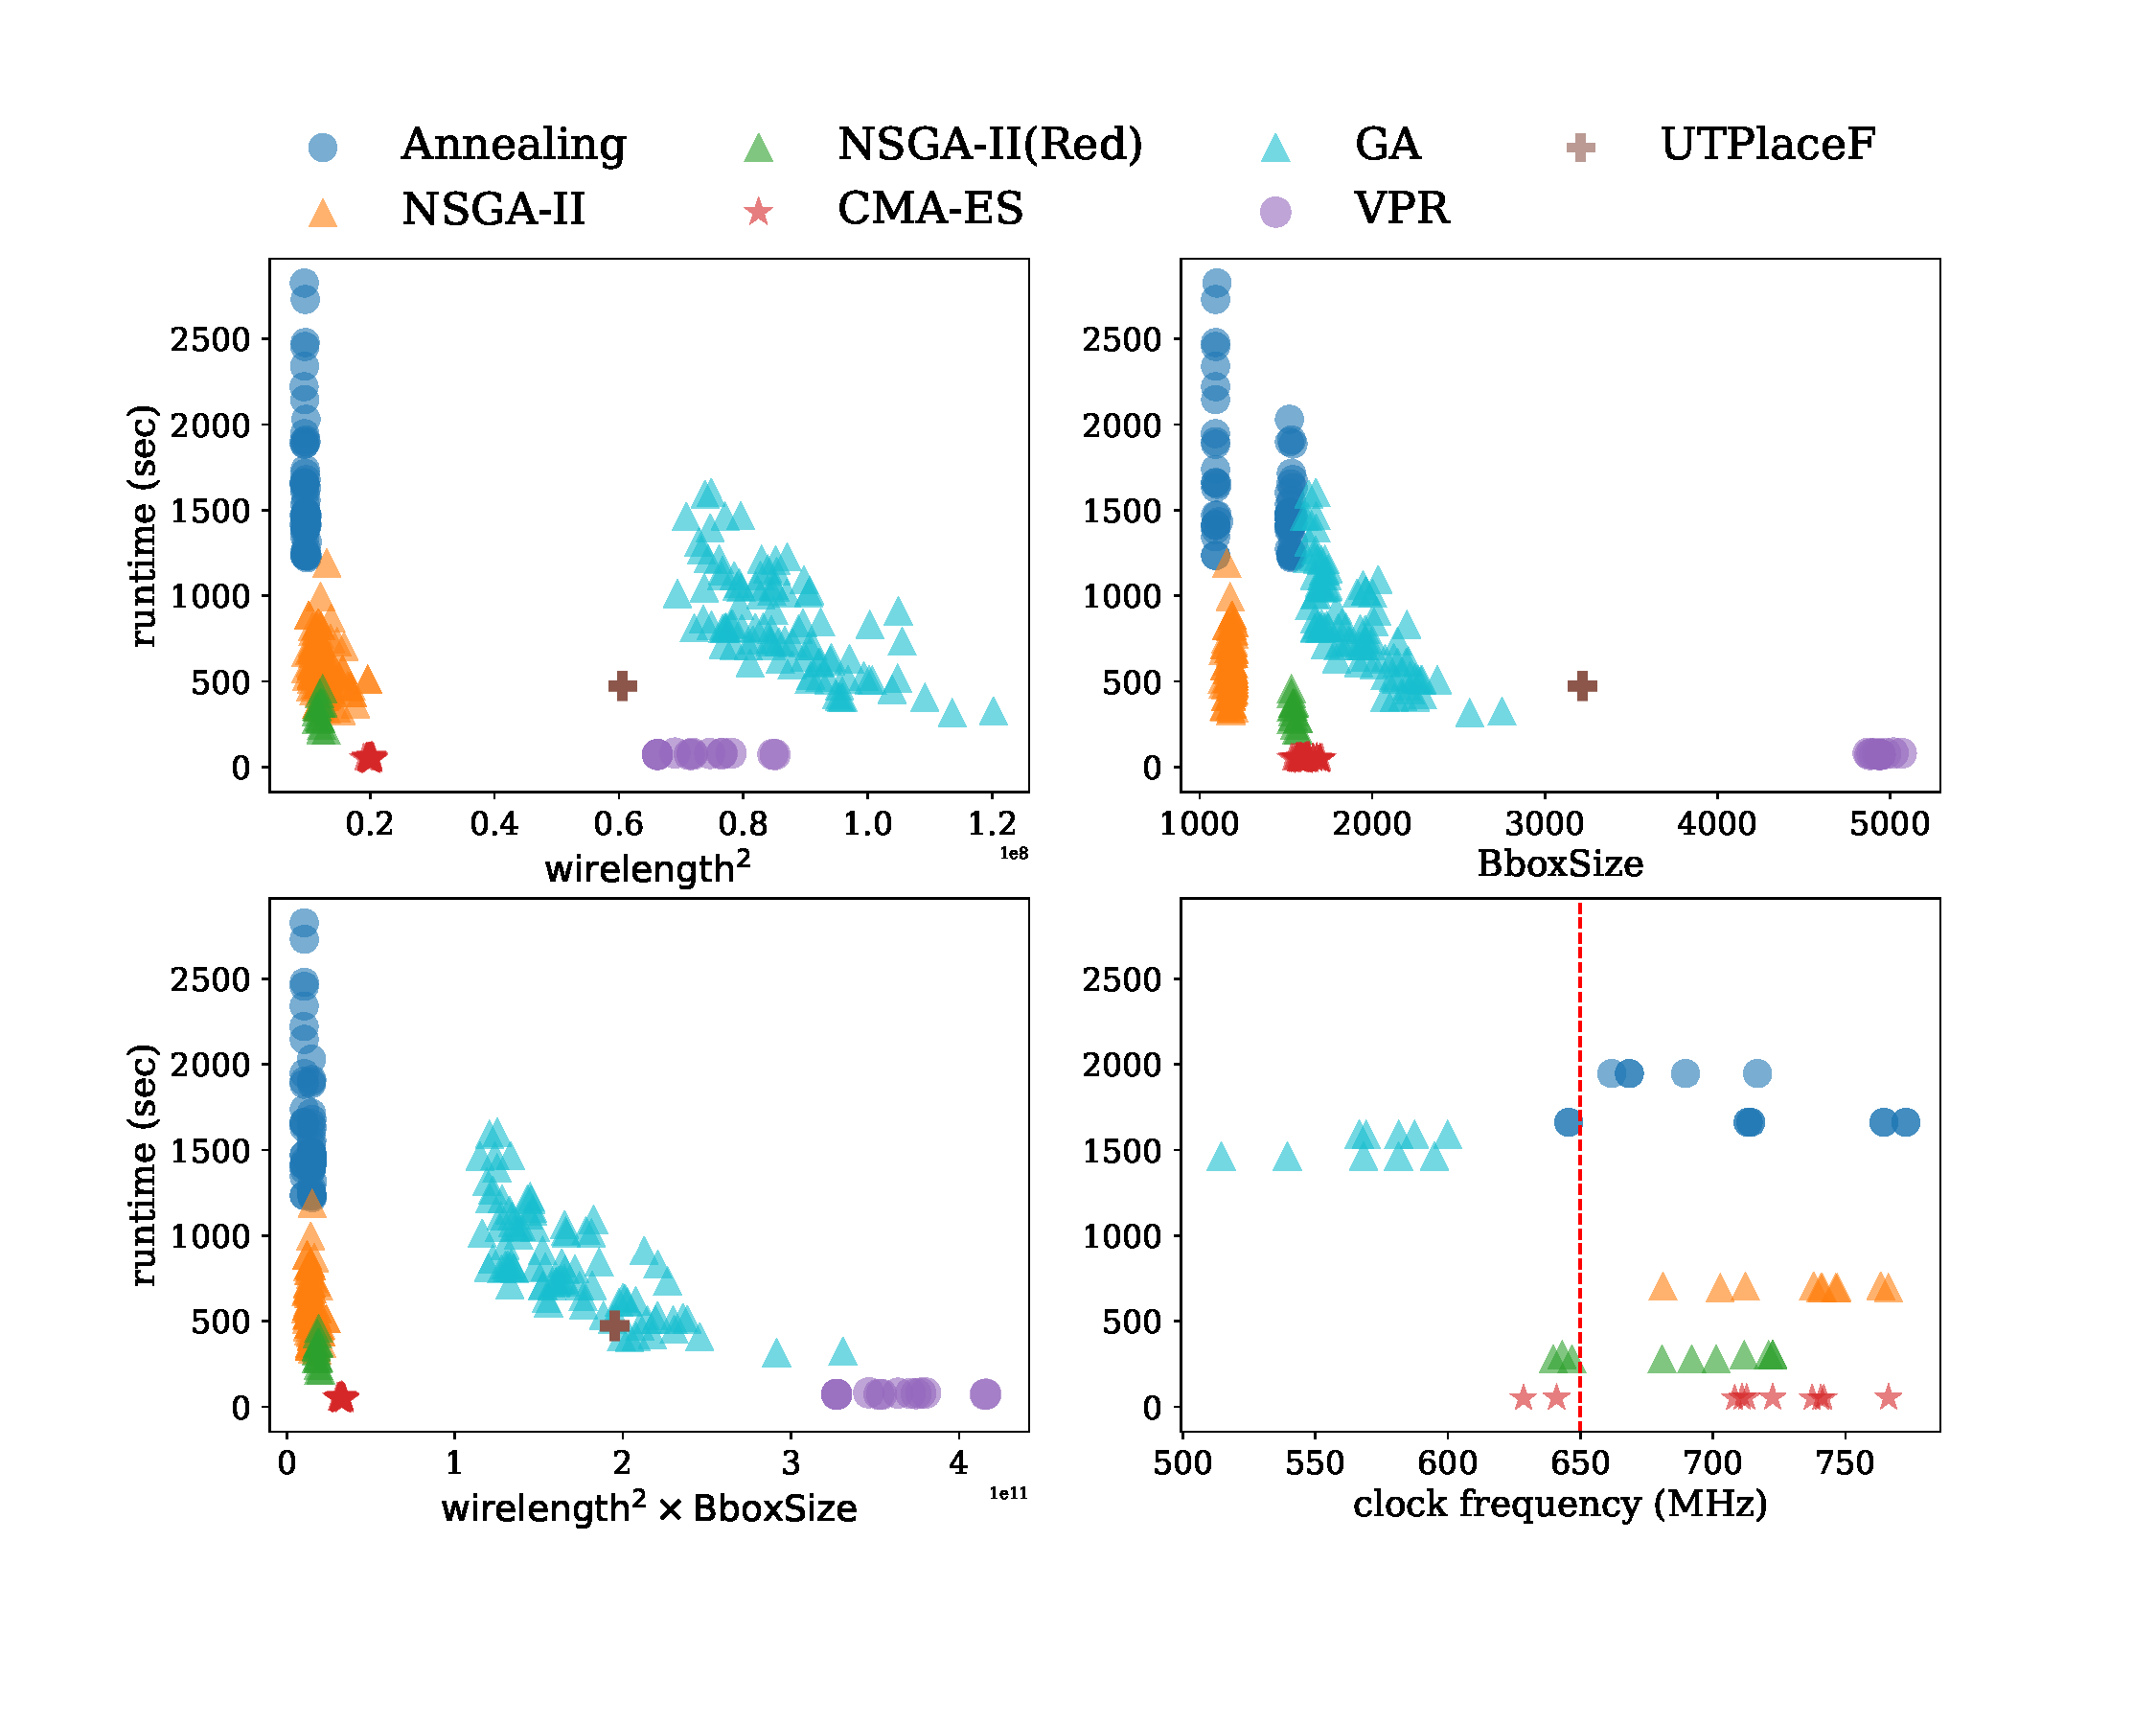
\includegraphics[width=\textwidth]{figure/objective-runtime}
	\caption{退火算法、NSGA-II、NSGA-II Reduced、CMA-ES、GA、UTPlaceF、VPR 的布局结果对比:目标函数值与时钟频率} 
	\label{fig:objective}
\end{figure}


% table of performance comparison
\begin{table*}[h]
% 	\caption{Runtime(avg), Wirelength(avg), Max BBox(avg), Pipelining
%   Registers(min), and Frequency(avg) for all methods. NSGA-II shows reduced
% genotype as well. Speeups and QoR improvements wins by Evolutionary algorithms
% also reported in \textcolor{red}{red}$\rightarrow$NSGA-II and \textcolor{olive}{green}$\rightarrow$CMA-ES 
% for each competitor algorithm (SA, GA, UTPlaceF, VPR, Manual).}
    
    \caption{平均运行时间,平均线长,平均最大边界框尺寸,达到650MHz最少所需流水线寄存器数目,以及平均时钟频率对比。
    左侧为本文提出的NSGA-II, NSGA-II Reduced, CMA-ES,右侧为对比算法。与各个对比算法相比每个指标的提升倍数在
    括号内标出,其中\textcolor{red}{红色}$\rightarrow$NSGA-II,\textcolor{olive}{绿色}$\rightarrow$CMA-ES}
	\label{table:comparison}
  \centering
  \begin{adjustbox}{width=1.1\textwidth,center}
  \begin{tabular}{c|c c| c c c c c}
	\toprule
  Method             & NSGA-II    	          & CMA-ES       & SA 					                                                                       & GA 			                                                                  & VPR     	                                                                & UTPlaceF 		                                                                   &  Manual \\
	\midrule
  Runtime (secs)     & 586 (323)		          & 51  		     &1577     (\textcolor{red}{2.7$\times$}, \textcolor{olive}{30.8$\times$})		        & 850 (\textcolor{red}{1.5$\times$}, \textcolor{olive}{16.7$\times$})		      & 76 (\textcolor{red}{0.13$\times$}, \textcolor{olive}{1.5$\times$})		    &  473 (\textcolor{red}{0.8$\times$}, \textcolor{olive}{9.3$\times$})            & 1--2 wks\\
  Wirelength  	     & 3.5K  (3.5K)   		    & 4.4K     		 &3.1K 	   (\textcolor{red}{0.9$\times$}, \textcolor{olive}{0.7$\times$})		          & 9.2K  (\textcolor{red}{2.6$\times$}, \textcolor{olive}{2.1$\times$})    		& 8.5K (\textcolor{red}{2.4$\times$}, \textcolor{olive}{1.9$\times$})   		&  7.8K  (\textcolor{red}{2.2$\times$}, \textcolor{olive}{1.8$\times$})          & 8.1K (\textcolor{red}{2.3$\times$}, \textcolor{olive}{1.8$\times$})  \\
  BBox      	       & 1183  (1543)   		    & 1606     		 &1387	   (\textcolor{red}{1.2$\times$}, \textcolor{olive}{0.9$\times$})		          & 1908  (\textcolor{red}{1.6$\times$}, \textcolor{olive}{1.2$\times$})   		  & 4941	(\textcolor{red}{4.1$\times$}, \textcolor{olive}{3.1$\times$})  		&   3218	(\textcolor{red}{2.7$\times$}, \textcolor{olive}{2.0$\times$})         & 1785 (\textcolor{red}{1.5$\times$}, \textcolor{olive}{1.1$\times$})  \\
  Pipeline Reg.		   & 256K  (273K) 		      & 273K	   		 &273K	   (\textcolor{red}{1.1$\times$}, \textcolor{olive}{1$\times$}) 	 	          & 323K	(\textcolor{red}{1.3$\times$}, \textcolor{olive}{1.2$\times$})   		  & -		                                                                      &   -                                                                            & 306K (\textcolor{red}{1.2$\times$}, \textcolor{olive}{1.1$\times$})   \\
  Frequency	(MHz)	 	 & 733  (688)   & 708 	 &711  (\textcolor{red}{0.97$\times$}, \textcolor{olive}{1.0$\times$})		        & 585 	(\textcolor{red}{0.80$\times$}, \textcolor{olive}{0.83$\times$})	& - 	      	                                                              & - 	                                                                           & 693 (\textcolor{red}{0.95$\times$}, \textcolor{olive}{0.98$\times$}) \\
	\bottomrule
	\end{tabular}
  \vspace{-0.2in}
\end{adjustbox}
\end{table*}

图\ref{fig:objective}展示了所有自动布局方法的运行时间,$wirelength^2$, 最大边界框尺寸,二者相乘$wirelength^2 \times BboxSize$,
以及Vivado timing report的时钟频率对比。表\ref{table:comparison}列出了图中内容的详细信息,以及进化算法相对对比实验各方面性能提高的
倍数。由性能对比的结果可以清晰得出以下几点结论:

\begin{itemize}
    \item NSGA-II比退火算法快大约2.7倍,同时可以得到小14.7\%的最大边界框尺寸,但是牺牲了大约12.9\%的线长。然而,在时钟频率一项
    NSGA-II仍然取得了优于退火的表现,这是由于相比退火的结果而言NSGA-II的优化结果更加稳定。
    \item CMA-ES 大约比退火快 {\bf 30倍}。尽管CMA-ES得到的最大边界框尺寸和线长相比退火的结果要差($\approx41$\%, $\approx16$\%),
    但CMA-ES仍然取得了与退火相当甚至更高的平均时钟频率(711 MHz)。
    \item NSGA-II Reduced 这一精简后的NSGA算法取得了相比退火快5倍的运行速度和相比完整NSGA-II快大约2倍的速度,但仅仅损失了2.8\%的
    时钟频率(688 MHz)且仍然高于URAM限制的650MHz最高运行频率。
    \item 与UTPlaceF和VPR相比,NSGA-II和CMA-ES两种进化算法在运行时间与结果质量上都有明显提高。
    \item 与单目标的遗传算法相比,NSGA-II多目标优化不但显著提升了结果质量,而且降低了运行时间。这说明本文的多目标优化设计可以加快
    优化过程,更有效地使算法收敛到近似全局最优解。
\end{itemize}

从表\ref{table:comparison}中的结果可以总结出,在50次实验中,NSGA-II和CMA-ES相比VPR和UTPlaceF得到了更优的结果质量(QoR),
相比于退火来说加速3--30倍,仅牺牲可以忽略的结果质量。对于实现时钟频率的目标650 MHz,NSGA-II比退火减少17K(约6\%)的流水
寄存器,同时相比手工布局节省50K(约16\%)的流水寄存器。


\subsection{收敛情况对比}

\begin{figure}[h]
    \hspace*{-1cm}
	\centering
	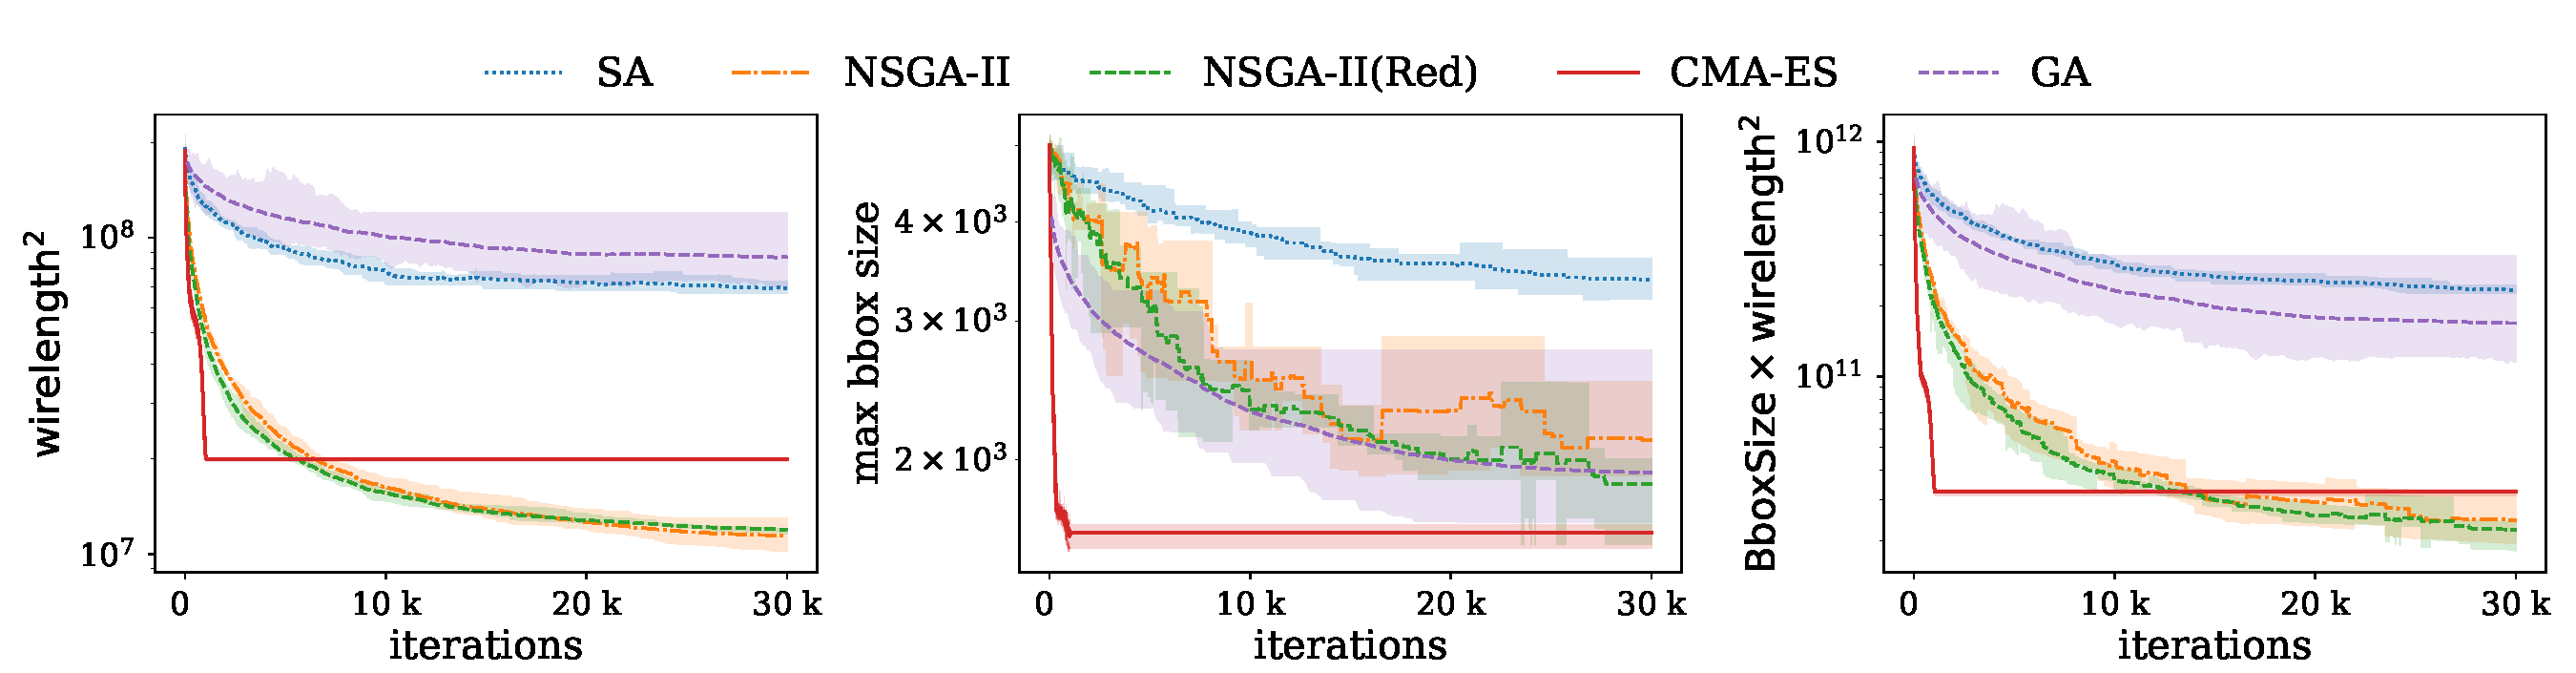
\includegraphics[width=1.1\textwidth]{figure/convergence}
	\caption{退火算法,NSGA-II,NSGA-II Reduced, CMA-ES,遗传算法的收敛进程对比} 
	\label{fig:converge}
\end{figure}

图\ref{fig:converge}画出了五种算法的收敛过程,包括两个目标函数和乘积的优化过程。可以观察到:
\begin{itemize}
    \item 退火收敛所需要的迭代次数最多,因此在30k的迭代次数以内目标函数降低幅度不明显;
    \item 单目标遗传算法的优化过程十分不稳定,尽管收敛较快但结果质量不高;
    \item 收敛所需要的迭代次数最少的,也是最稳定的算法是CMA-ES,在不到2000个迭代次数内已完成收敛,得到的结果质量较高;
    \item NSGA-II和NSGA-II Reduced 在15K个迭代次数之后布局结果质量超过CMA-ES。可以观察到去掉2个子基因型对
    NSGA-II的收敛速度影响不大,由此可以判断NSGA-II Reduced得到的加速来源于省略的解合法化过程。
\end{itemize}


\subsection{流水线级数对时钟频率的影响}

\begin{figure}[h]
	\centering
	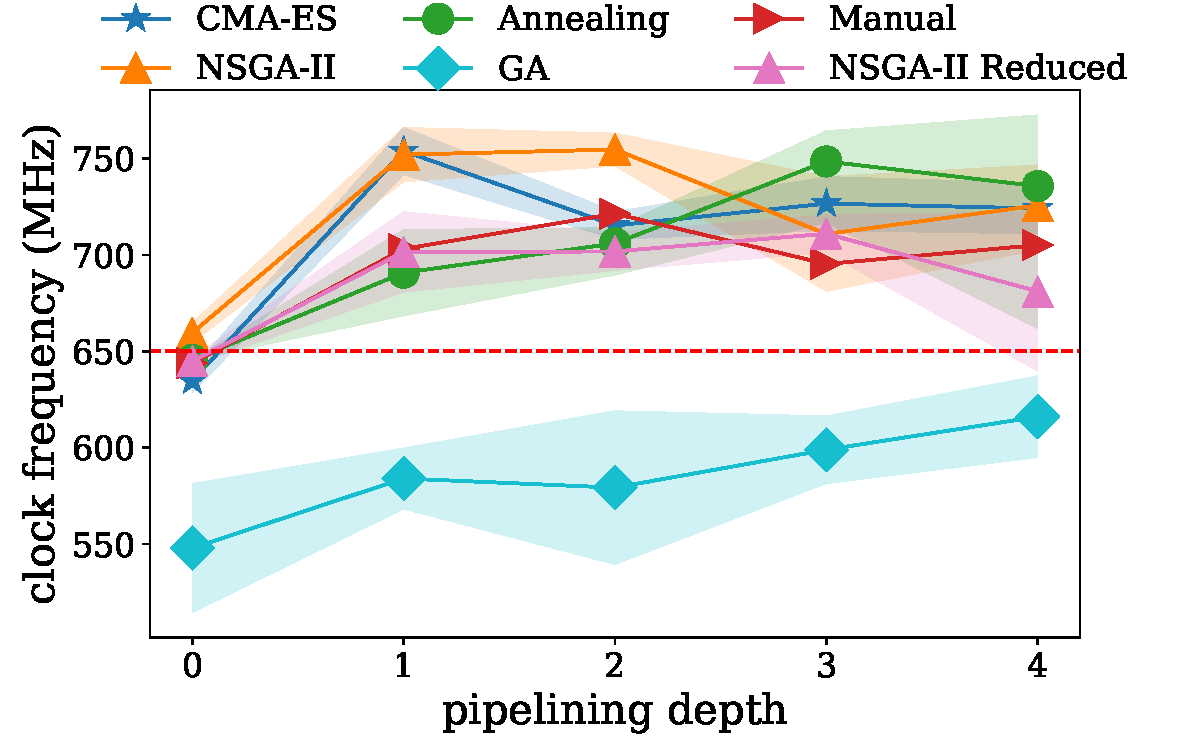
\includegraphics[width=0.7\textwidth]{figure/frequency_depth}
	\caption{六种布局方法时钟频率随流水线级数的变化} 
	\label{fig:freq_depth}
\end{figure}

图\ref{fig:freq_depth}画出了十次优化实验中CMA-ES,NSGA-II,NSGA-II Reduced,遗传算法,退火算法以及手动布局的
时钟频率相对于流水线级数的变化。NSGA-II在不需要额外流水线的情况下达到了650 MHz的实际运行频率上限,而退火算法,CMA-ES和
手动布局至少需要1级流水线。对于规模越大的设计,节省一级流水线带来的寄存器减少就越大。本文在VU11P的480个卷积单元实验中,
NSGA-II节省的一级流水线来了17K--50K个流水线寄存器的减少,极大减轻了布线压力。

同时观察到NSGA-II,CMA-ES仅需两级流水线即可达到750 MHz的极高时钟频率,而退火则需要3--4级流水线,
手工布局更是无法达到这样的高频率。这启示着在未来的架构改进和设计改进中如果设计支持750 MHz以及以上的高频率运行,NSGA-II和CMA-ES
更加有潜力。



\subsection{布局的迁移学习}

\begin{table}[h!]
    \caption{硬核布局在不同FPGA的迁移学习性能: VU3P, VU11P 作为初始设备}
    \label{table:port}
    \centering
    \begin{adjustbox}{width=0.8\columnwidth,center}
    \begin{tabular}{c|c c c c c}
      \toprule
  \multirow{2}{*}{Device}     & Design Size 		& Impl.Runtime 		& Frequency 	 & \multicolumn{2}{c}{Placement Runtime}    			\\ \cline{5-6}
                                 & (conv units)		& (mins.)				& (MHz)			 & 	Scratch (s)			& 	Transfer (s)				\\
      \midrule
      \emph{xcvu3p}  			& 123				&	46.4			& 718.9			 & 428.3				& - 							\\
      \emph{xcvu5p}  			& 246				&   56.9				& 677.9	 		 & 396.0				& 55.7 	(\textcolor{red}{7.1$\times$})							\\
      \emph{xcvu7p}  			& 246			    &   55.1				& 670.2	 		 & 345.4				& 44.2 	(\textcolor{red}{7.8$\times$})							\\
      \emph{xcvu9p}  			& 369	   			&   58.4				& 684.9	 		 & 316.5				& 45.5 	(\textcolor{red}{7$\times$})							\\ 
      \midrule
      \emph{xcvu11p} 			& 480	      	    &	65.2          	& 655.3	 		 & 695.9				& -								\\	
      \emph{xcvu13p} 			& 640        	    & 	69.4   			& 653.2	 		 & 704.9				& 58.8	(\textcolor{red}{12$\times$})			\\
      \bottomrule
    \end{tabular}
    \vspace{-0.1in}
    \end{adjustbox}
  \end{table}

RapidLayout 能够在不同资源比例、不同硬核列分布、不同大小的FPGA设备上得到高质量的布局结果,对布局结果在不同设备之间
的迁移学习更加快了布局的搜索进程。RapidLayout的迁移学习功能将已有设备上的硬核布局结果作为在新设备上布局的初始化参考,
从而不同比例和列分布的新设备上达到比随机初始化更快的收敛结果。本文将UltraScale+系列FPGA根据硬核列数量分为两组,如
表\ref{table:port}所示。分组的依据是硬核资源列的数目需要相等或近似,因为初始化将布局结果转化为基因型时,基因型的大小与硬核资源
的列数有关。在这两组中,我们分别令VU3P和VU11P作为初始设备进行布局优化,之后通过迁移学习将布局结果
迁移到其他设备。从表\ref{table:port}中可以总结出,使用迁移学习可以为布局优化过程加速7--12倍。

RapidLayout 的SLR复制功能使得大型FPGA的布局布线时间不随资源数量增大而线性增大。这是因为在RapidLayout的工作流中,
最耗时的部分是单个SLR内的布线过程,而一旦一个SLR布线完成,则可以直接将该结果用于整个FPGA,所以FPGA的尺寸增大不会
导致运行时间相应增大。从表\ref{table:port}的结果可以发现,从VU3P到VU13P,FPGA可容纳卷积计算单元的数目由
123增大到640,也就是增加了5.2倍;而其实现时间仅有46分钟增加到了69分钟,仅增大了1.5倍。

\newpage

\subsection{布局结果展示}

\begin{figure}[h]
	\centering
	\subfloat[Vivado内置解析布局引擎结果,因阻塞严重无法完成布线]{
		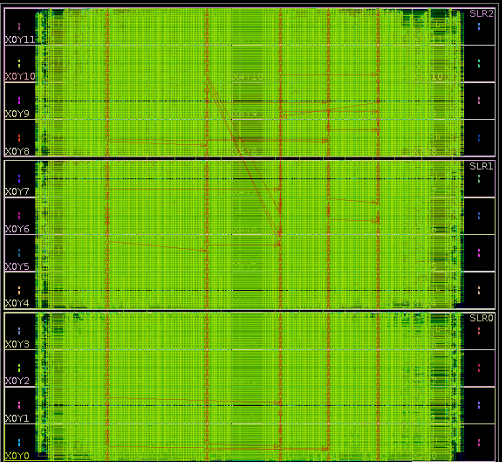
\includegraphics[width=0.3\textwidth, height=0.5\textwidth]{figure/vivado-placed.png}
	}
	\hfill
	\subfloat[由Vivado实现的手工布局结果,耗时5--6小时]{
		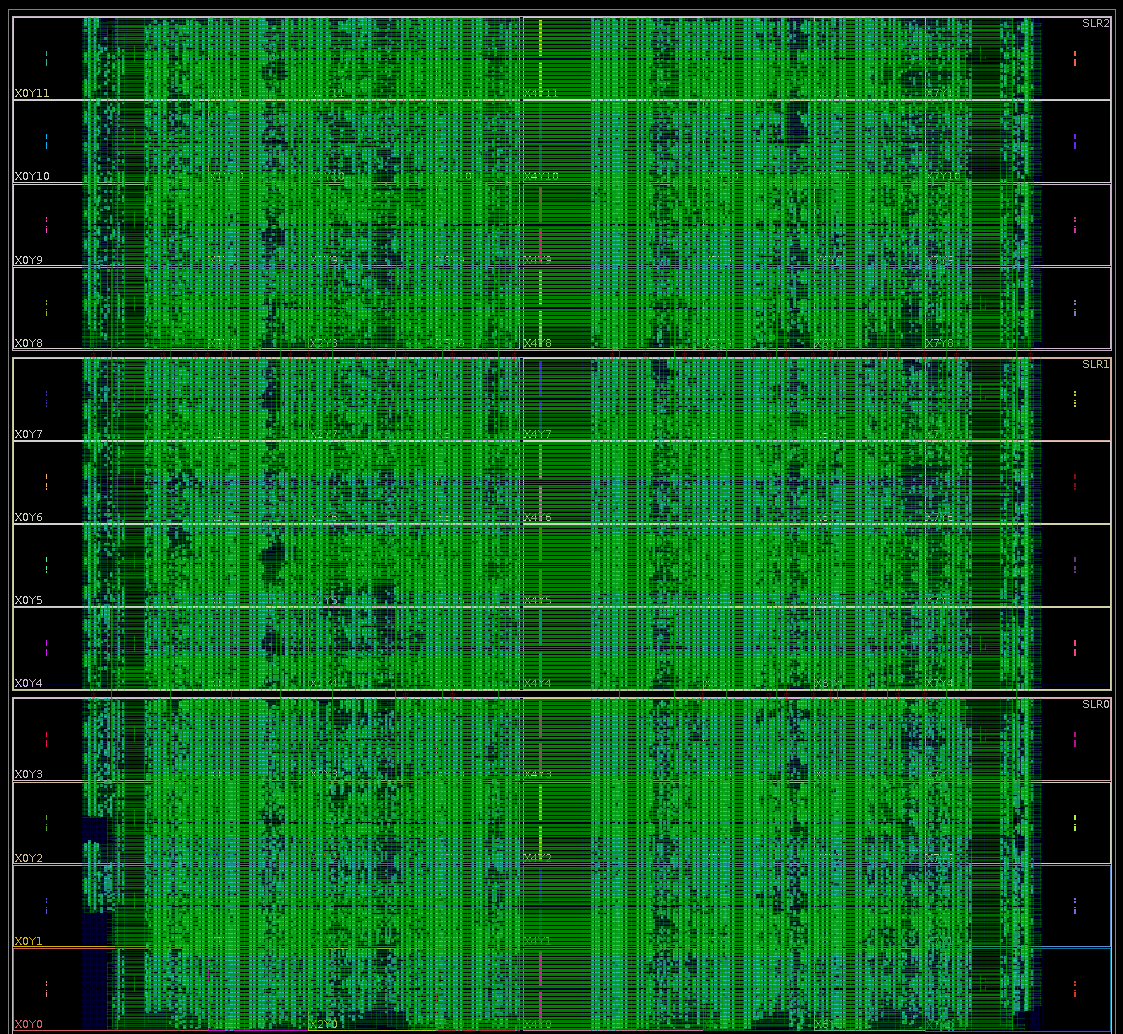
\includegraphics[width=0.3\textwidth, height=0.5\textwidth]{figure/manual-placed.png}
	}
	\hfill
	\subfloat[RapidLayout的自动布局布线,耗时 $\approx$1 小时] {
		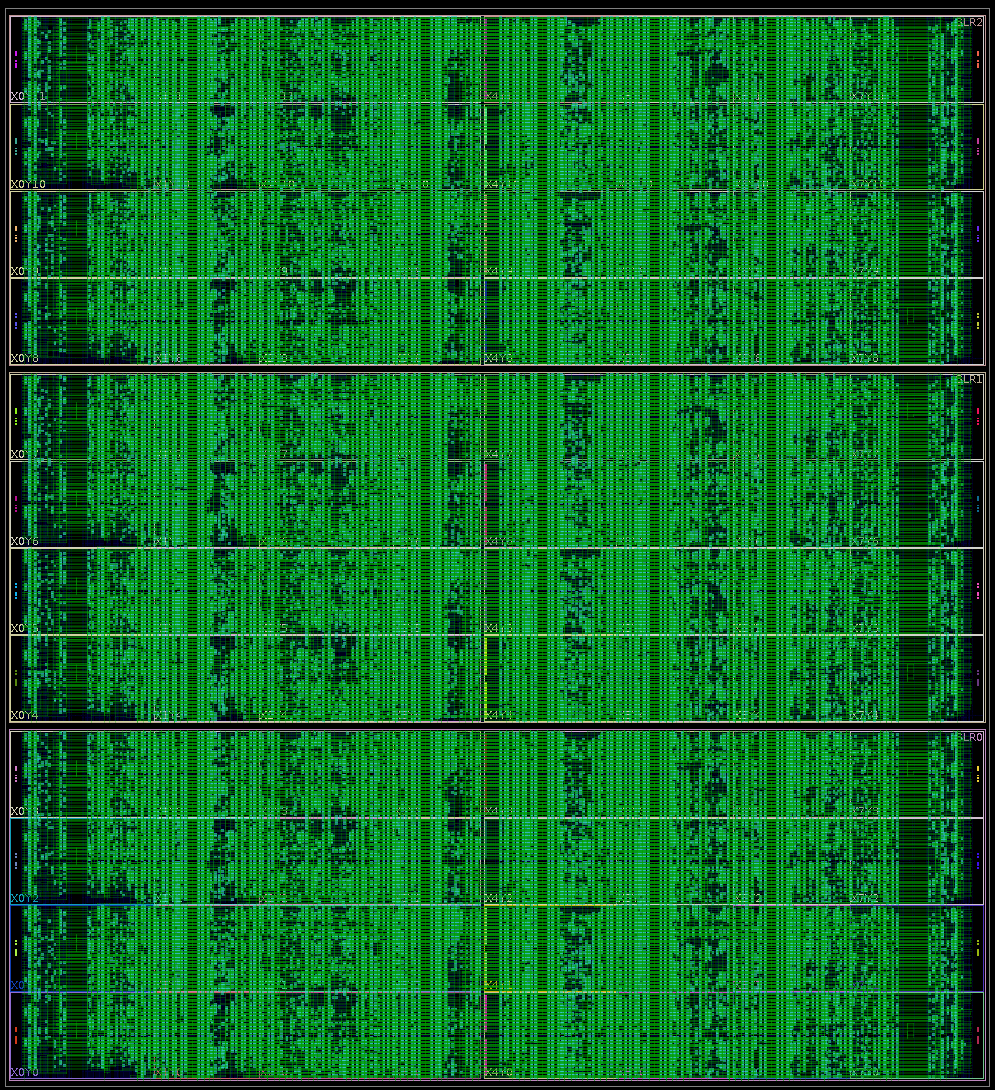
\includegraphics[width=0.3\textwidth, height=0.5\textwidth]{figure/rapidlayout-placed.png}
	}
	\caption{
   480个卷积运算单元在Xilinx UltraScale+ VU11P FPGA 上的布局结果
    }
	\label{fig:overview}
\end{figure}

\section{本章小结}

本章首先介绍实验中涉及的UltraScale+ VU3P-13P FPGA器件,使用的对比算法,
然后介绍实验的编程实现、运行环境、参数确定、敏感性分析等实验细节。
其次,本章设计了多种可视化方法展示与state-of-the-art方法
的性能、收敛过程对比。验证了多目标进化算法在布局任务上相对其他方法的
优势:相对退火算法3--30倍的搜索时间加速,比最先进解析布局方法更小的
边界框尺寸与线长,相比手工布局节省6\%-16\%的流水寄存器等。
本章详细讨论了流水线级数对时钟频率的影响,从结果中体现出进化算法的另一个优势:
仅需较少的流水线级数即可达到700~MHz以上的超高时钟频率。
最后,本章评估RapidLayout的迁移学习性能并展示布局结果,体现了
基于SLR布局布线结果复用的方式对大规模设计的速度优势。









































































% \chapter{基于多线索操纵的图像颜色编辑应用}
% 内容概括 \cite{Zuo10}

% \section{多线索操纵图像颜色编辑框架设计}
% 多线索操纵的交互式颜色传递框架集合了基于颜色聚类分割、基于图像修补的边界矫正、梯度保持优化和颜色分布映射等多种手段。……

% \section{多线索操纵图像颜色编辑框架具体实现}
% 多线索操纵图像颜色编辑框架集合了全局图像颜色编辑和局部图像颜色编辑功能。……

% \section{多线索操纵图像颜色编辑实验结果分析}
% 下面将分别给出全局以及局部图像颜色编辑的实验结果对比,并进行分析。……

% \section{本章小结}
% 在本章中,我们提出一种基于多线索操纵的图像颜色编辑方法,介绍图像编辑框架流程。本文采用Mathworks的MATLAB 2010a作为实验平台,结合附带的图像处理工具箱进行算法验证,同时使用MATLAB的GUI设计工具实现了交互式的操作程序,使得实验过程更加直观。实验结果表明,本章所提出的图像编辑框架具有比较强的可操作性和比较理想的处理结果。由于使用 GUI交互操作的方式,因此,用户有了更多的操控自由。


